\documentclass[10pt]{article}
\usepackage[utf8]{inputenc}
\usepackage{graphicx}
\usepackage[portuguese]{babel}

\title{Robôs Domésticos \& Robôs Industriais}
\date{Abril de 2023}


\usepackage[sorting=none]{biblatex}
\bibliography{references}
\PassOptionsToPackage{hyphens}{url}
\usepackage{url}


\setcounter{biburllcpenalty}{7000}
\setcounter{biburlucpenalty}{8000}

\begin{document}

\maketitle
\begin{center}
    \Large Universidade de Évora
\end{center}

\renewcommand\abstractname{Abstract}
\begin{abstract}
O tema que pretendemos abordar é sobre os robôs domésticos e industriais, visto que nos últimos anos têm tido uma enorme evolução, apesar de essa evolução passar despercebida aos olhos de todos nós.

Pretendemos explicar o que são os robôs domésticos e os robôs industriais, bem como as suas respetivas histórias e evoluções ao longo do tempo. O nosso objetivo é também expor algumas vantagens e desvantagens de cada um desses tipos de robôs, tanto no nosso dia a dia quanto em um nível mais geral.

Outra razão pela qual escolhemos este tema, além de estar relacionado com a nossa área e de ser interessante, é a sua influência que tem vindo a ter no mercado financeiro. O desenvolvimento de robôs domésticos e industriais têm impulsionado o crescimento de empresas que investem nessa tecnologia e têm atraído a atenção de investidores em todo o mundo.

Por último, planeamos apresentar alguns dos exemplos mais relevantes tanto para robôs domésticos como industriais, incluindo fotos. Além disso, vamos explicar as suas funções, as capacidades e características específicas de cada um, bem como o seu funcionamento.
\end{abstract}

\begin{center}
\textbf{Keywords} \\
robôs - robôs domésticos - robôs industriais - mercado financeiro
\end{center}

%\section{Introdução}
%\hspace{\parindent}O objetivo deste artigo consiste em analisar a significativa evolução dos robôs nos últimos anos, a qual muitas vezes passa despercebida aos olhos de muitos.
%Assim sendo, e uma vez que o tema dos robôs é muito amplo, decidimos escolher os dois tipos de robôs mais conhecidos e fazer uma análise comparativa entre eles: os robôs domésticos e os robôs industriais.
%
%Temos como tópicos da análise a definição e as características de cada um dos robôs, a sua evolução ao longo dos anos, as vantagens e desvantagens de cada um, o impacto de cada um no mercado financeiro.


\section{O que é um robô? E o que é a robótica?}

\hspace{\parindent}Um robô é um dispositivo eletrónico programável capaz de executar tarefas de forma autónoma ou semi-autónoma. Estes dispositivos podem ser controlados por um computador ou por um software específico.

Já a robótica é a área da tecnologia que se dedica ao estudo, desenvolvimento e criação de robôs. Esta área de atuação inclui diversas disciplinas como a eletrónica, a mecânica, a inteligência artificial, a programação e a engenharia. A robótica tem vindo a evoluir de forma significativa nas últimas décadas, e atualmente desempenha um papel fundamental em diversos setores da sociedade.

\section{O que é um robô Doméstico?}
\hspace{\parindent}Um robô doméstico\cite{whatare} é, tal como o nome indica, um robô destinado a realizar as tarefas domésticas, ou seja, para ajudar as pessoas com as tarefas diárias, como limpar a casa, aspirar o chão, entre outras atividades, sendo uma das razões para que este tipo de robô, seja cada vez mais populares.

Ademais, estes robôs podem ainda ser utilizados em outros ramos, como o da educação, entretenimento e terapia.

Mesmo que a maioria dos robôs domésticos seja simplista, alguns estão conectados, não só a redes domésticas WiFi, mas também a ambientes inteligentes, tornando-os assim autónomos em alto grau. 

\section{O que é um robô Industrial?}
\hspace{\parindent}Os robôs industriais\cite{robotnik_2022} são máquinas projetadas e programadas para executar e automatizar tarefas repetitivas e por vezes perigosas que são tradicionalmente realizadas por pessoas, realizando-as com precisão e rapidez, sendo mais eficazes. 

Os robôs industriais são capazes de executar diversos tipos de tarefas, como montagem de produtos, soldagem, pintura, inspeção, embalagem e muitas outras. Estes são normalmente equipados com sensores, atuadores e controladores, e podem operar de forma autónoma ou ser controlados por operadores humanos. 

Este tipo de robôs são usados em várias indústrias, nomeadamente a indústria automóvel, eletrónica, aeroespacial, entre outras, e tem o objetivo de aumentar a produtividade, melhorar a qualidade do produto e aumentar a segurança no local de trabalho.

\section{História e Evolução}

\subsection{Robôs}
\hspace{\parindent}A primeira introdução de robôs ocorreu durante a Revolução Industrial, com o objetivo de processar materiais e produzir bens. Este evento foi um marco na história da humanidade, pois melhorou significativamente a qualidade de vida do Homem.

Naquele tempo, havia muitas dúvidas em relação aos robôs, principalmente sobre a possibilidade de eles se revoltarem contra os humanos. Foi então que o escritor Isaac Asimov, preocupado com a segurança dos robôs, idealizou três leis fundamentais (posteriormente quatro) para a robótica, com o objetivo de controlar e limitar o comportamento dos robôs\cite{wikipedia_2022}:

\begin{itemize}
    \item \textbf{1ª Lei:} Nenhum robô pode ferir um ser humano, ou por inação, que o ser humano sofra algum mal;
    \item \textbf{2ª Lei:} Todos os robôs devem obedecer às ordens que são dadas pelos seres humanos, exceto se essa ordem entrar em conflito com a 1ª Lei;
    \item \textbf{3ª Lei:} Qualquer robô deve proteger a sua própria existência, desde que essa proteção não entre em conflito com a 1ª e 2ª Leis.
    \item \textbf{Lei Zero:} Mais tarde, Asimov acrescentou a \textbf{"Lei Zero"}, que está acima das outras todas, e refere que nenhum robô pode causar mal à humanidade, ou que por omissão, permita que a humanidade sofra algum mal.
\end{itemize}

\subsection{Robôs Domésticos}
\hspace{\parindent}Os robôs domésticos\cite{history} tiveram a sua origem na década de 1980, quando os primeiros robôs de serviço começaram a ser comercializados para uso em residências.

Um dos primeiros robôs domésticos a ser criado chamava-se \textit{HERO}. Existiram quatro modelos deste robô, sendo o primeiro o \textit{HERO 1}, usado na educação, para ensinar programação e robótica. A versão \textit{HERO JR} foi criada para uso próprio, visto que era mais acessível que a primeira e foi comercializado principalmente para escolas. Já o modelo \textit{HERO 2000} tinha uma melhor capacidade de processamento que as duas primeiras, mas era mais complexo. A última versão (\textit{Arm Trainer}) focava-se mais na área industrial.

\begin{figure}[h]
\centering
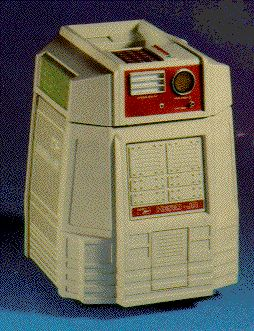
\includegraphics[width = 3.5cm]{img/hero.jpg} 
\label{figura:1}
\caption{Robô Hero.}
\end{figure}

Com o passar dos anos e o com o avanço da tecnologia, os robôs domésticos foram melhorados com recursos adicionais, tais como o reconhecimento de voz, capacidade de aprendizagem e adaptação às necessidades dos utilizadores, bem como a conectividade com dispositivos inteligentes em casa, o que permitiu limpar autonomamente a casa, ajudar na cozinha (é o caso da Bimby), ter assistentes pessoais, como a Alexa da Amazon. Estas melhorias permitiram ter também robôs que ajudassem pessoas com necessidades especiais ou robôs de companhia para idosos.

Com a constante evolução da tecnologia, é provável que os robôs domésticos continuem a desenvolver-se e a desempenhar um papel cada vez mais importante nas nossas vidas quotidianas.

\subsection{Robôs Industriais}
\hspace{\parindent}Em 1954, o inventor americano George Devol criou o primeiro robô industrial, chamado Unimate, um dispositivo de duas toneladas que transferia objetos autonomamente de um lugar para outro, como mostra a figura abaixo\cite{wevolver}.
\\
\begin{figure}[h]
\centering
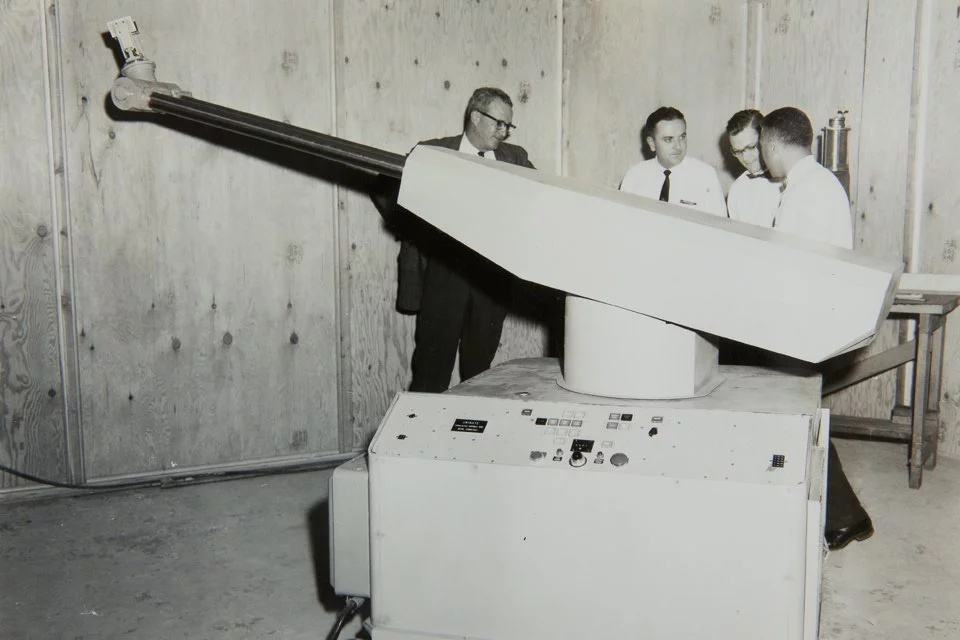
\includegraphics[width = 5cm]{img/robind.png}
\label{figura:2}
\caption{Representação do primeiro robô industrial, o Unimate.}
\end{figure}
\\

Desde então, com o avanço de sensores, da eletrónica e de software, as capacidades dos robôs industriais expandiram consideravelmente para incluir tarefas complexas, como soldar, pintar, montar, embalar e testar, tudo realizado com velocidade, precisão e repetibilidade.

Durante o final dos anos 1960 e início dos anos 1970, com a crescente demanda pela automatização de tarefas intensivas em mão-de-obra na indústria, a robótica industrial passou a concentrar-se no manuseio de materiais e no trabalho de precisão, levando ao desenvolvimento de robôs elétricos de menor porte, mas com controles avançados, microprocessadores e motores miniaturizados, facilitando tarefas como apertar parafusos e porcas.

Em meados da década de 1980, houve um aumento significativo do interesse pela robótica. Os engenheiros começaram a entender os robôs como as "máquinas do futuro" e a ampliar os seus limites, para apoiar o desenvolvimento industrial e assim, alcançar uma maior competitividade na indústria. Foi durante este período que a base do robô industrial atual foi lançada, com a incorporação de sensores avançados e sistemas rudimentares de visão de máquina.

A partir do começo dos anos 2000, os progressos na robótica industrial têm sido fortemente impulsionados pelo avanço do software. Novos campos, como \textit{Machine Learning} e Inteligência Artificial, estão agora a avançar as fronteiras do que os robôs podem fazer, dando-lhes a capacidade de aprender, melhorar e tomar decisões sem direção ou orientação humana. É expectável que, nos próximos anos, à medida que os robôs industriais se tornem mais avançados, sejam capazes de assumir tarefas ainda mais complexas e executá-las com uma eficiência que supere as capacidades humanas.


\section{Exemplos dos robôs}
\subsection{Domésticos}
\hspace{\parindent}Com os progressos tecnológicos, nomeadamente na área da robótica, foram sendo criados cada vez mais robôs que pudessem ser usados por qualquer pessoa como ferramentas de dia a dia. Exemplos disso são a criação de aspiradores automáticos, de assistentes virtuais e até \textit{'animais'} (robóticos) de estimação.

% aspiradores automaticos
Existem diversos tipos de aspiradores automáticos, mas nem todos têm as mesmas capacidades, e estes têm vindo a melhorar cada vez mais. Inicialmente estes eram limitados, pois tinham uma baixa autonomia e dependiam de caminhos pré-programados para conseguir contornar objetos. No entanto, com a evolução dos sensores e introdução de câmaras, estes aspiradores conseguiam mapear o ambiente à sua volta navegar mais eficientemente.

Ao longo do tempo estes continuaram a evoluir, obtendo capacidades como poderem ser calendarizados, poderem ser controlados remotamente através de \textit{apps mobile}, focarem-se em áreas mais sujas através de sensores, mapear automaticamente as divisões da casa, podendo mais tarde escolher limpar apenas certas divisões, e claro foram melhorando as suas capacidades de limpeza.

Alguns robôs mais avançados até possuem IA e ML incorporados otimizando ainda mais o processo de limpeza.

% assistentes virtuais
Os assistentes virtuais, também conhecidos por \textit{Smart Home Hubs} têm vindo a evoluir rapidamente nos últimos anos, devido principalmente aos avanços na IA, reconhecimento de voz e IoT (Internet das Coisas). \\
Estes aparelhos oferecem imensa personalização, são multitarefas, podem ser integrados com terceiros, 'aprendem' com o utilizador permitindo recomendações inteligentes e mais direcionadas aos seus interesses. Todas estas capacidades permitem ter uma 'casa inteligente', costumizada particularmente aos gostos de cada utilizador.

% 'animais' de estimação/companhia (aibo)
Durante a CES 2018, uma das maiores feiras de tecnologia do mundo, foi lançado o
\emph{Aibo}, um robô que tentava imitar ao máximo um cão de estimação. A sua função não era executar nenhuma tarefa específica, mas sim fazer o papel de um animal de estimação e de melhor amigo.

Este robô doméstico possui inteligência artificial, tendo a capacidade de reconhecer e afeiçoar-se ao dono, pois reconhece caras e sons. Desenvolvido
pela \emph{Sony}, o \emph{Aibo} funciona a bateria e tem uma duração de aproximadamente duas horas. Por ser um modelo relativamente recente e não ter tido muita procura (seria um produto muito caro) ainda não chegou ao mercado.

\begin{figure}[!h]
\centering
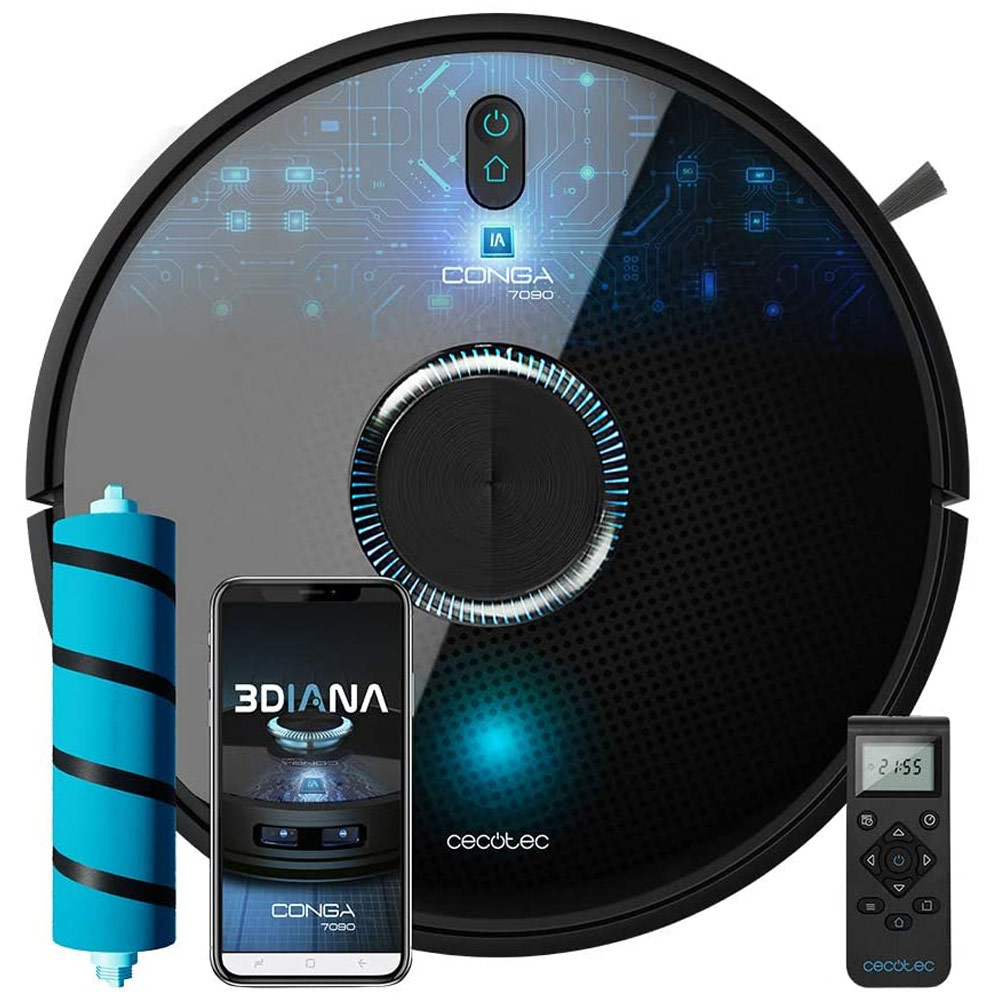
\includegraphics[width = 3.5cm]{img/aspirador.jpg}
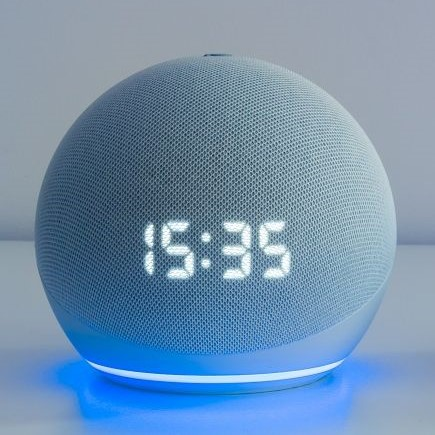
\includegraphics[width = 3.5cm]{img/assistente-virtual.jpg}
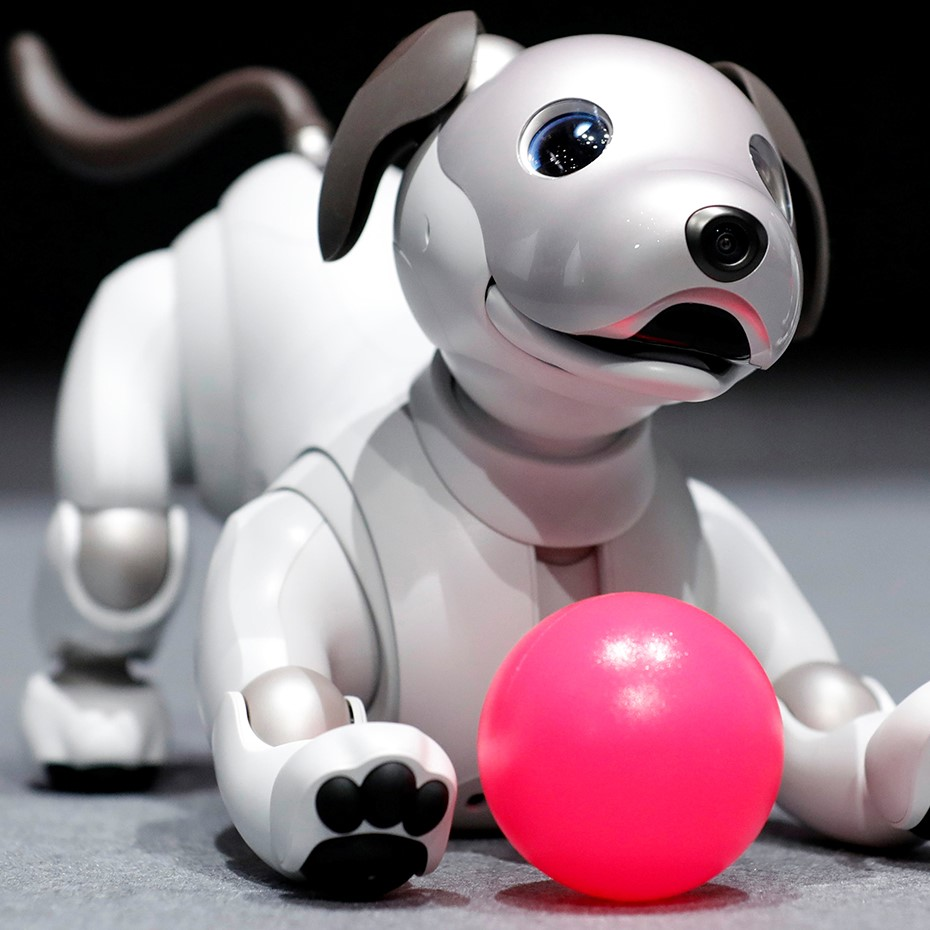
\includegraphics[width = 3.5cm]{img/aibo.jpg}
\label{Robôs Boston Dynamics}
\caption{Aspirador automático, Assistente Virtual e Animal Robótico.}
\end{figure}


\subsection{Industriais}
\hspace{\parindent}Os robôs industriais mais comuns costumam ser usados em armazéns ou construção de produtos maiores a partir da junção de peças mais pequenas. Estes costumam ser braços mecânicos ou outras máquinas capazes de montar e lidar com materiais com características muito distintas. Este tipo de robôs pode ser usado em imensas indústrias, como construção, montagem, pesquisa, mineração, segurança pública e até entertenimento.

Uma das empresas que se especializa em robótica é a norte-americana \emph{Boston Dynamics}, que já tem 3 robôs comercializáveis - \emph{Stretch}, \emph{Spot} e \emph{Spot Arm} [\ref{Robôs Boston Dynamics}].

% Stretch
O robô \emph{Stretch}\cite{stretch} é um robô muito sofisticado e versátil projetado para automação de armazéns. Este robô consiste em um aparelho móvel, com um braço extensível e uma garra que pode lidar com uma ampla variedade de objetos, sendo ideal para tarefas como empilhar objetos, mover paletes e organizar objetos de armazéns em geral. Com a sua tecnologia de percepção, e a sua precisão, consegue navegar em ambientes complexos, e lidar autonomamente com várias tarefas num armazém em constante mudança, ajudando a melhorar a eficácia e a produtividade do local.

% Spot e Spot Arm
O robô \emph{Spot}\cite{spot} da \textit{Boston Dynamics} é um robô de \textit{'quatro patas'} altamente móvel e autónomo. Possui pernas articuladas e sensores que permitem a sua navegação em ambientes complexos. O \emph{Spot} também pode ser usado para vários efeitos, como a inspeção de locais de difícil acesso, monitorização de ambientes perigosos e transporte de carga leve. 

Já o \emph{Spot Arm}\cite{spot-arm} é um acessório ao \emph{Spot}, que consiste num braço robótico. Este permite que o \emph{Spot} tenha capacidades adicionais para a manipulação de objetos e realização de tarefas que requerem extra destreza e precisão, permitindo-o agarrar, levantar e manipular diversos objetos.

\begin{figure}[!h]
\centering
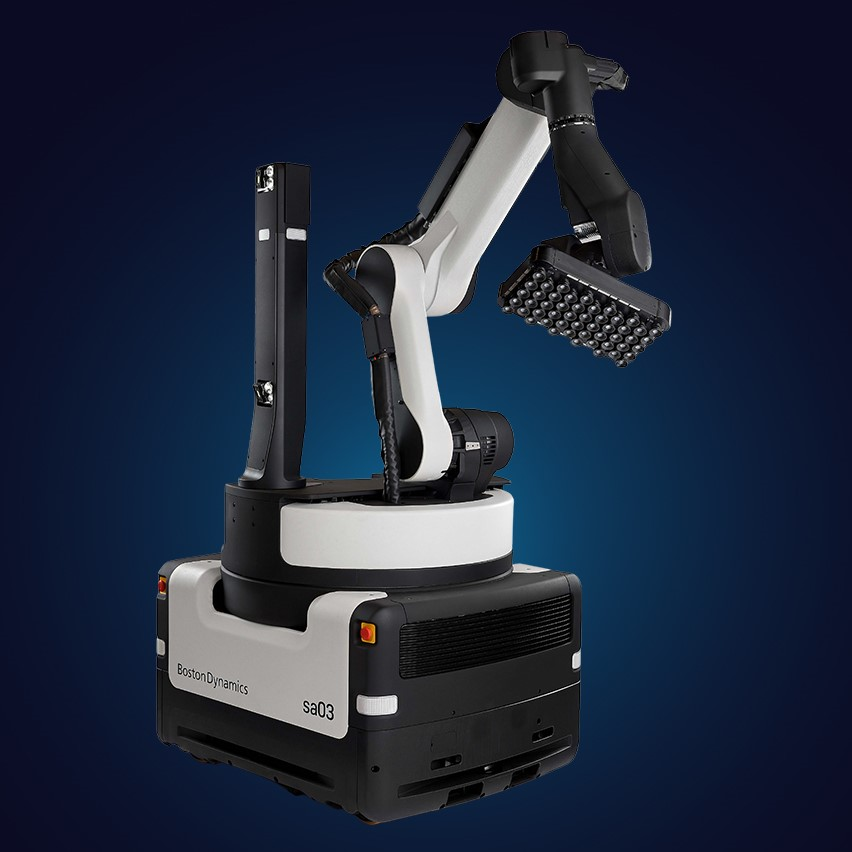
\includegraphics[width = 3.5cm]{img/stretch.jpg}
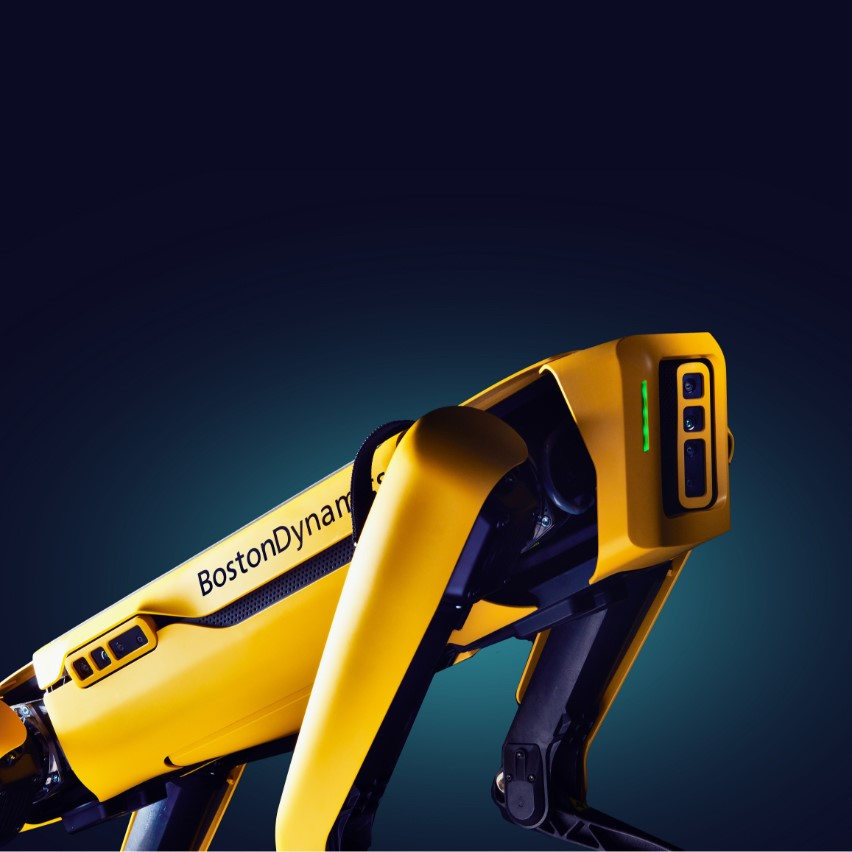
\includegraphics[width = 3.5cm]{img/spot.jpg}
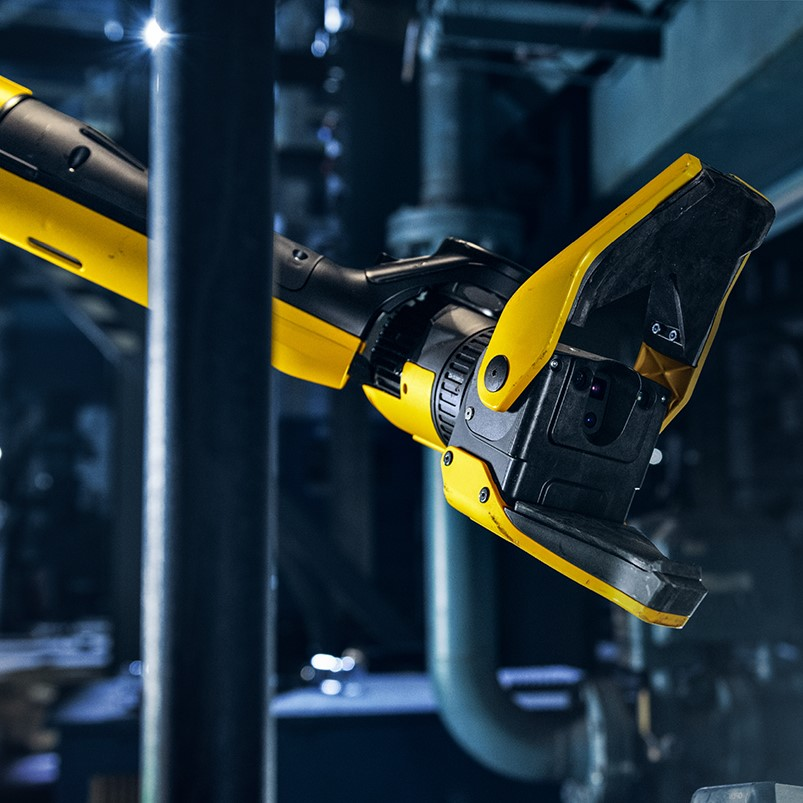
\includegraphics[width = 3.5cm]{img/spot-arm.jpg}
\label{figura:4}
\caption{Robôs Stretch, Spot e Spot Arm, respetivamente.}
\end{figure}

Por curiosidade, esta empresa possui também um robô humanoide chamado \emph{Atlas}, que ainda não foi comercializado. O objetivo deste robô é estudar e ultrapassar os limites da tecnologia atual, e poderia ser utilizado em operações de resgate ou serviços de emergência, podendo sobreviver em ambientes aos quais os seres humanos não conseguiriam aceder.


\section{Vantagens e Desvantagens}
\subsection{Vantagens dos Robôs Domésticos\cite{advantages}}

\begin{enumerate}
    \item Os robôs domésticos têm a capacidade de executar uma série de tarefas domésticas, o que permite poupar tempo.
    \item Este tipo de robôs também podem ser utilizados como ferramentas educacionais, ou seja, as crianças podem aprender sobre programação, eletrónica e mecânica, de forma lúdica e interativa. Outra vantagem é desenvolver habilidades importantes, como a resolução de problemas, o pensamento crítico, o trabalho em equipa e comunicação.
    \item Os robôs domésticos podem ser programados para trabalhar em horários específicos e podem ser controlados remotamente, o que proporciona uma maior conveniência para os utilizadores.
    \item Estes robôs têm um papel importante com idosos e pessoas com deficiências. Podem ajudá-los com tarefas diárias e também ser utilizados para treinamento e reabilitação, como em fisioterapia para ajudar na recuperação da mobilidade e coordenação. Além disso, os robôs de companhia podem fornecer interação social, reduzindo assim, a solidão e o isolamento social. 
    \item Por fim temos a segurança. Existem muitos robôs domésticos que têm a função de vigiar a casa e alertar os proprietários sobre atividades suspeitas, como ladrões ou problemas com fugas de água ou gás. Alguns modelos estão equipados com câmaras de segurança e sensores de movimento, o que permite que os proprietários monitorizem remotamente as suas casas em direto, com o auxílio do telemóvel.
\end{enumerate}

\subsection{Desvantagens dos Robôs Domésticos\cite{advantages}}

\begin{enumerate}
    \item O custo, muitos modelos de robôs domésticos são caros e podem não estar disponíveis para todas as famílias.
    \item O risco de privacidade: alguns modelos de robôs domésticos têm câmeras e microfones embutidos, o que pode levantar preocupações com privacidade e segurança de dados.
    \item A falta de humanidade, embora os robôs possam fornecer interação social, eles não têm a mesma empatia e compreensão que um ser humano pode oferecer.
    \item A sua dependência da tecnologia, os robôs domésticos podem ser difíceis de reparar quando danificados e também como dependem da eletricidade e da conexão com a internet, torna-se problemático em caso de falhas no sistema.
\end{enumerate}

\subsection{Vantagens dos Robôs Industriais\cite{stevens_2022}}

\begin{enumerate}
    \item Os robôs industriais têm como vantagem a eficiência, uma vez que são capazes de realizar tarefas repetitivas por longos períodos de tempo sem precisar de pausas ou descansos. Isso leva a um aumento da produtividade e a uma redução dos custos de produção.
    \item Este tipo de robôs têm capacidade de realizar tarefas com uma precisão e rapidez muito maior do que os seres humanos, o que é especialmente importante em processos de fabricação que requerem medidas exatas e consistência.
    \item Podem ser usados para executar tarefas que são perigosas para os trabalhadores, como manusear materiais tóxicos ou trabalhar em ambientes extremos. Isso ajuda a garantir a segurança dos trabalhadores, eliminando a exposição a potenciais riscos.
    \item Têm a capacidade de serem programados para realizar diversas tarefas e operar em diferentes ambientes, o que os torna adequados para uma variedade de aplicações de fabricação. Ademais, são menos propensos a erros do que seres humanos, fazendo com que os produtos tenham uma menor probabilidade de possuir defeitos.
    \item Os custos de produção podem ser reduzidos, já que menos trabalho humano é necessário, resultando em produtos mais acessíveis.
\end{enumerate}

\subsection{Desvantagens dos Robôs Industriais\cite{stevens_2022}}

\begin{enumerate} 
    \item O investimento inicial para adquirir robôs industriais é significativo, o que pode ser um obstáculo para pequenas e médias empresas.
    \item Requerem manutenção regular para garantir o seu desempenho adequado e prolongar a sua vida útil. Isto pode ser caro e requer pessoal especializado.
    \item Falta de criatividade, embora os robôs industriais sejam altamente precisos e eficientes em tarefas repetitivas, não são capazes de lidar com situações imprevistas ou improvisar soluções para problemas que não foram previamente programados.
    \item O uso crescente de robôs industriais pode levar à perda de empregos em algumas indústrias, à medida que as empresas se tornam mais automatizadas e menos dependentes de trabalhadores humanos.
\end{enumerate}


\newpage


\section{A influência dos Robôs no mercado financeiro}
\hspace{\parindent}Os benefícios da utilização dos robôs no mercado de ações são diversos\cite{market}, podendo substituir os humanos em certas profissões, aumentando a rapidez na execução de tarefas, bem como a sua capacidade de produzir ou funcionar 24/7, permitindo às empresas aumentarem as suas produções por exemplo. Além disso, o avanço tecnológico permite que hajam cada vez mais e melhores robôs.

\subsection{Robôs Domésticos}
\hspace{\parindent}O mercado de robôs domésticos\cite{international} tem vindo a crescer cada vez mais e este crescimente não parece vir a alterar-se nos próximos anos. De acordo com a \textit{International Federation of Robotic Report 2019}, espera-se que as vendas unitárias de robôs domésticos aumentem 46\% em média por ano, com mais de 55 milhões de unidades vendidas em 2022. Além disso, os valores de venda dos robôs domésticos aumentaram em 15\% para 3,7 mil milhões de euros. 

As inovações tecnológicas, no que diz respeito à cognição, interação e manipulação, tornaram a robótica doméstica mais atraente. Tecnologia e outros fornecedores de componentes têm sido fundamentais para o avanço do ecossistema robótico. Por exemplo, em abril de 2019, investigadores da Universidade da Califórnia desenvolveram um robô que usa inteligência artificial (IA) para realizar tarefas humanas intrincadas, como ajudar a dobrar roupas ou fazer uma chávena de café. 

O aumento da automação em eletrodomésticos, o aumento dos custos de mão de obra e as crescentes preocupações com a segurança estão a impulsionar a procura por robôs domésticos no mundo inteiro. 

Outro conceito que tem vindo a ser cada vez mais falado é casa inteligente. Em 2019, \emph{Temi}, uma empresa responsável por um dos maiores websites de transcrições de áudio para texto, fez parceria com a \emph{Amazon Alexa} para projetar robôs inteligentes, móveis e pessoais movidos a IA. A \emph{Samsung} e a \emph{LG Electronics} estão também a investir extensivamente no desenvolvimento e lançamento de novos produtos robóticos domésticos. Também estão a ser desenvolvidos robôs sociais para integração na vida doméstica e como companheiros interativos. Observando o potencial do mercado, as \emph{startups} que oferecem soluções de robôs domésticos estão também a atrair investidores internacionais. No entanto, o alto custo do equipamento acaba por limitar a taxa de adoção deste tipo de robôs.

\newpage

\begin{figure}[h]
\centering
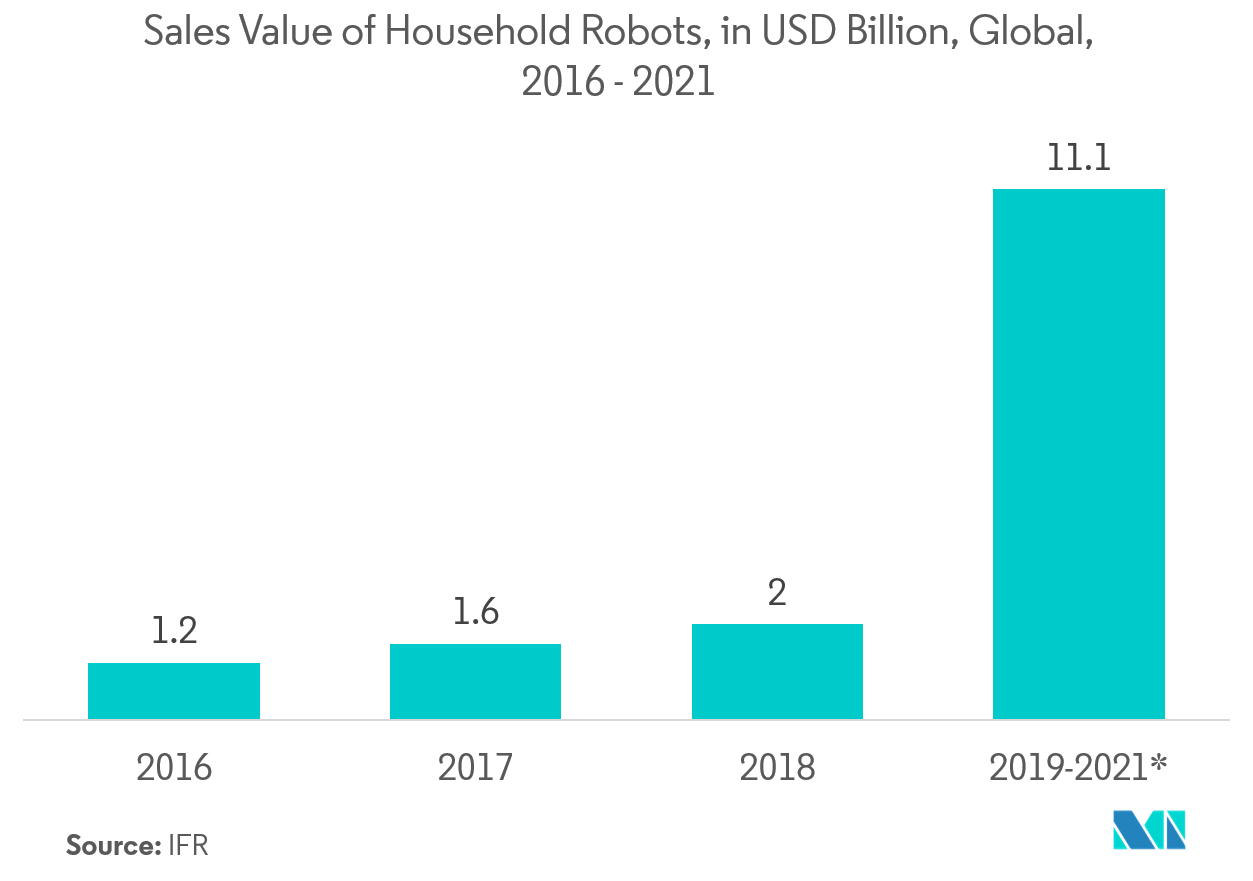
\includegraphics[width = 7cm]{img/grafico-domesticos.png}
\label{Venda de robôs domésticos}
\caption{Venda de Robôs Domésticos entre 2016 e 2021}
\end{figure}

Como podemos ver no gráfico da figura 5 [\ref{Venda de robôs domésticos}], o número de vendas de robôs domésticos entre os anos 2019 e 2021 foi muito superior ao número de vendas dos anos anteriores, registando aproximadamente 11 biliões de dólares em vendas, sensivelmente o dobro do valor nos três anos anteriores a 2019.


\subsection{Robôs Industriais}
\hspace{\parindent}A Ásia tem atualmente o maior mercado de robôs industriais\cite{internacional2}, com 74\% de todos os novos robôs em 2021, nomeadamente na China e no Japão. Isto representa um crescimento, não muito acentuado, comparativamente a 2020, cuja percentagem era de apenas 70\%.

Na China, houve um aumento de unidades vendidas em 2021 - aproximadamente 268 mil robôs - resultando num crescimento de 51\% relativamente a 2020. No mesmo espaço de tempo, estavam operacionais mais de 1 milhão de robôs, mostrando o rápido aumento no uso destes robôs na China, e assegurando o primeiro lugar no uso destes robôs na Ásia.

O Japão segue em segundo lugar, com cerca de 47 mil unidades instaladas em 2021, totalizando pouco mais de 393 mil unidades operacionais no mesmo ano. Este é também o país que mais constrói e exporta este tipo de robôs, tendo um máximo de cerca de 186 mil unidades exportadas apenas em 2021.

 Na Europa, os países que mais se destacam no mercado dos robôs industriais são a Alemanha e a Itália. Em 2021, o número total destes robôs operacionais na Alemanha era de quase 246 mil robôs, ficando pouco abaixo da China, e cerca de 89 mil unidades na Itália.
 
 Por fim, no continente americano, o país que mais se destaca são os Estados Unidos, no entanto a demanda deste tipo de robôs tem vindo a diminuir ligeiramente desde 2016 a 2021. Apesar disso, este continente ainda totaliza mais de 50 mil unidades apenas em 2021, sendo a indústria automóvel a que mais utiliza estes robôs industriais.

Durante dois anos desde 2019 a utilização dos robôs industriais parou de crescer, possivelmente devido ao impacto que a pandemia teve em quase todas as maiores indústrias, mas voltou a crescer em 2021, mantendo-se em crescimento desde então.

 Em 2021 foi registado o \emph{'pico'} da instalação de novos robôs industriais, aproximadamente 517 mil robôs instalados em fábricas no mundo inteiro. O relatório da \emph{World Robotics} mostra que isto representa um aumento no uso destes robôs de 31\% por ano. Em outubro de 2022, o número de robôs operacionais existentes em todo o mundo rondava os 3 milhões e meio de unidades.
\\
\\
\begin{figure}[h]
\centering
\label{Instalação de robôs industriais}
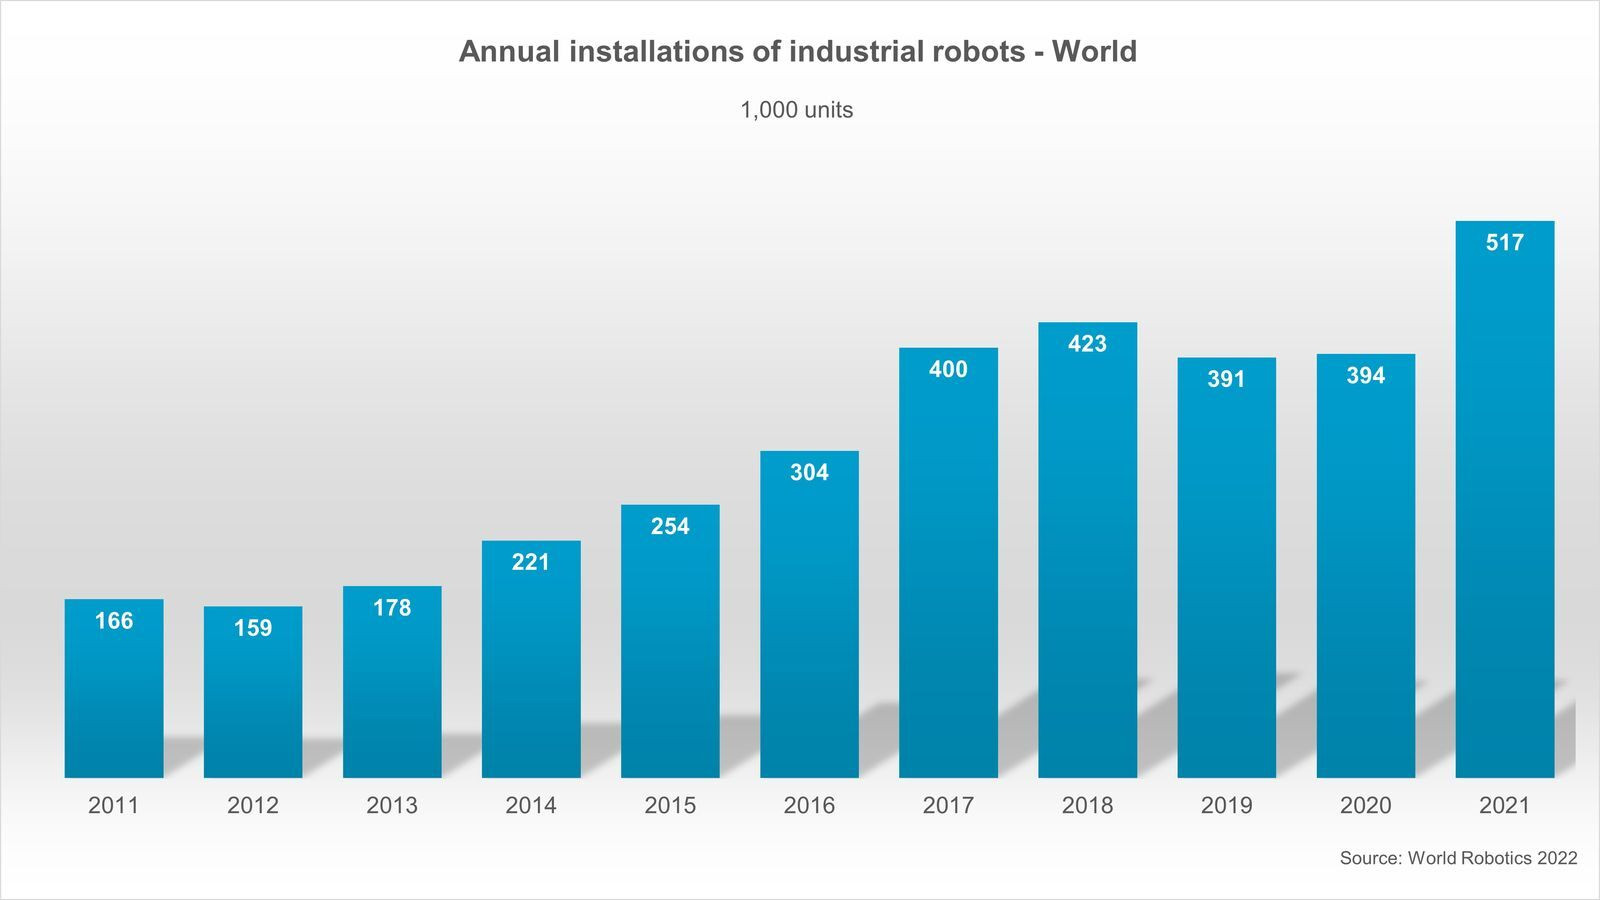
\includegraphics[width = 7cm]{img/grafico-industriais.jpg}
\caption{Instalação de Robôs Industriais entre 2011 e 2021}
\end{figure}

No gráfico da figura 6 [\ref{Instalação de robôs industriais}], conseguimos observar que o número de indústrias que começaram ou aumentaram a utilização de robôs industriais tem vindo a aumentar praticamente em cada ano, tendo mais que triplicado num espaço de tempo de 10 anos.


\section{Conclusão}
\hspace{\parindent}Podemos concluir que os robôs, tanto domésticos como industriais, foram uma grande passo para a automatização de tarefas na indústria e para auxílio pessoal.

Cada vez mais surgem novas tecnologias e com isto podem ser feitas melhorias aos robôs já existentes ou até criar novos, que sejam mais completos e eficientes a fazer as suas tarefas.

Prevemos também um aumento das vendas de robôs para uso pessoal e um aumento na utilização de robôs em diversas indústrias, resultando num aumento da procura e maior mercado financeiro.

\newpage

\printbibliography[title=Referências]  



\end{document}


